\documentclass[a4paper, 12pt]{article}

\usepackage{amsmath}
\usepackage{amssymb}
\usepackage{titlesec}

\usepackage{tikz}
\usetikzlibrary{trees}

\setlength{\parindent}{0pt}
\setlength{\parskip}{1em}

\titlespacing*{\section}{0pt}{0pt}{0pt} % {left}{before}{after}
\titlespacing*{\subsection}{0pt}{0pt}{0pt}
\titlespacing*{\subsubsection}{0pt}{0pt}{0pt}

\begin{document}

\title{Dynamic Programming}
\author{LQR471814}
\maketitle

\section{Basic ideas}

Any dynamic programming problem has a certain objective, minimizing cost, maximizing profits, maximizing utility, etc... The function that describes this objective is known as the \emph{objective function}.

Information about the current situation required to make a correct decision is known as \emph{state}. (ex. To gauge how much to spend, you must know how much you have. Therefore wealth $W$ would be one of the state variables)

Variables chosen by the agent are called \emph{chosen variables}, these are decisions made based on \emph{state variables} which influence the next state (though next state is often also influenced by stuff outside the \emph{chosen variables}).

Dynamic programming describes the optimal chain of decisions by finding a rule that determines the most optimal decision given any possible of the state. (ex. If consumption only depends on wealth, you would want to find a function $c(W)$ which gives the optimal consumption for any degree of wealth) This is known as a \emph{policy function}.

\section{Formalization}

Suppose $x_{t}$ is the state at a time $t$, the initial state being $x_{0}$.

At any point the set of possible actions is defined as $a_{t} \in \Gamma(x_{t})$, where: 1) $a_{t}$ are the particular values for a set of control variables (variables that influence the next state) 2) $\Gamma(x_{t})$ is the set of actions that can be taken at state $x_{t}$.

State changes from $x$ to a new state $T(x, a)$ when action $a$ is taken.

The objective function that calculates the optimality of a given action $a$ on a state $x$ is $F(x, a)$.

Finally, we can define the \emph{value function} (the function that describes the best possible value of the objective as a function of state $x$) like follows.

\[
  V(x) = \underset{a \in \Gamma(x)}{\text{max}}\{F(x, a) + V(T(x, a))\}
\]

\emph{Interpretation:} The value function is the maximum value of the objective function (given the current $a$) added to the value function of the next state (given the current $a$) for all $a$ in $\Gamma(x)$.

Usually we are given $x_0$, $T$, $F$, and $\Gamma$ as part of the problem description and are tasked with finding $V(x)$ (the most optimal value possible for a given starting state) and $a(x)$ (the optimal decision to make at a given state).

\section{Examples}

\subsection{Optimal stopping problem}

Suppose a person is evaluating potential employment opportunities for the next 10 years ($t = 1, 2, 3, ...$).

At each value $t$, they may encounter a choice between a ``good'' job offering $\$100$ in salary or a ``bad'' job offering $\$44$, each with an equal probability of being offered. 

\begin{itemize}
  \item Pick the available job offered.
  \item Reject the offer and wait till the next year.
\end{itemize}

The question then becomes, what are the choices that should be made over the 10 year period to maximize money obtained?

This can be solved by reasoning backwards from $t=10$:

\begin{enumerate}
  \item At $t = 10$ the total earnings from accepting a ``good'' job is $\$100$; the value of accepting a ``bad'' job is $\$44$; the total earnings from rejecting the available job is $\$0$. Therefore, if they are still unemployed in the last period, they should accept whatever job they are offered at that time for greater income.
  \item At $t = 9$, the total earnings from accepting a ``good'' job is $2 \times 100 = 200$ because that job will last for two years. The total earnings from accepting a ``bad'' job is $2 \times 44 = 88$. The total expected earnings from rejecting a job offer are $0$ now plus the value of the next job offer, which will either be $44$ with $\frac{1}{2}$ probability or $100$ with $\frac{1}{2}$ probability, for an average (``expected'') value of $\frac {\$100+\$44}{2}=\$72$. Therefore, the job available at $t=9$ should be accepted.
  \item At $t=8$, the total earnings from accepting a ``good'' job is $3\times \$100=\$300$; the total earnings from accepting a ``bad'' job is $3\times \$44=\$132$. The total expected earnings from rejecting a job offer is $\$0$ now plus the total expected earnings from waiting for a job offer at $t=9$. As previously concluded, any offer at $t=9$ should be accepted and the expected value of doing so is ${\frac {\$200+\$88}{2}}=\$144$. Therefore, at $t=8$, total expected earnings are higher if the person waits for the next offer rather than accepting a ``bad'' job.
\end{enumerate}


By continuing to work backwards, it can be verified that a ``bad'' offer should only be accepted if the person is still unemployed at $t=9$ or $t=10$; a bad offer should be rejected at any time up to and including $t=8$. Generalizing this example intuitively, it corresponds to the principle that if one expects to work in a job for a long time, it is worth picking carefully.

\subsubsection{Math interpretation}

\[
\begin{aligned}
  x &= (o, j, t) \\
  x_{o} &\in \{44, 100\} \\
  x_{j} &\in \{\text{has job}, \text{no job}\} \\
  \{x_{t} &\in \mathbb{Z} | 1 \leq x \leq 10\}
\end{aligned}
\]

\begin{itemize}
  \item $x$ is the state.
  \item $x_{o}$ is the amount of money you would earn if you had a job.
  \item $x_{j}$ is your employment status.
  \item $x_{t}$ is the current time.
\end{itemize}

\[
\begin{aligned}
  a(x) \in \Gamma(x) = \begin{cases}
    \{\text{no change}\}, & x_{j} = \text{has job} \\
    \{\text{no change}, \text{take job}\}, & x_{j} = \text{no job}
  \end{cases}
\end{aligned}
\]

\begin{itemize}
  \item $a(x)$ is the optimal action to take for a given state $x$.
  \item $\Gamma(x)$ is the possible actions that can be taken for a given state $x$.
\end{itemize}

\[
\begin{aligned}
  T(x, a) = \begin{cases}
    (x_{o}, \text{has job}, x_{t} + 1), & a = \text{take job} \\
    \begin{cases}
      (\text{rand}(100, 44), x_{j}, x_{t}+1), & x_{j} = \text{no job} \\
      (x_{o}, x_{j}, x_{t}+1), & x_{j} = \text{has job}
    \end{cases}, & a = \text{no change}
  \end{cases}
\end{aligned}
\]

\begin{itemize}
  \item $T(x, a)$ defines the next state for a given current state $x$ and chosen action $a$.
\end{itemize}

\[
\begin{aligned}
  F(x, a) = \begin{cases}
    x_{o}, & a=\text{take job} \\
    \begin{cases}
      x_{o}, & x_{j}=\text{has job} \\
      0, & x_{j} = \text{no job}
    \end{cases}, & a=\text{no change}
  \end{cases}
\end{aligned}
\]

\begin{itemize}
  \item $F(x,a)$ is the objective function that determines how optimal taking the given action $a$ on the current state $x$ is.
\end{itemize}

\[
  V(x)=\underset{a \in \Gamma(x)}{\text{max}}\{F(x,a)+V(T(x,a))\}
\]

We can see that we are given $x$, $\Gamma(x)$, $T(x, a)$, and $F(x, a)$ from the problem. Our job now, is to determine what $V(x)$ and $a(x)$ are, most commonly through processes of induction.

\subsubsection{Solving for the equations}

We'll use the technique of backwards induction to derive the equations $V(x)$ and $a(x)$.

This involves starting from a base case, then branching off from that base case and seeing what the commonalities are.

\textbf{Base cases}

\[
\begin{aligned}
  V((100, \text{no job}, 10)) &= \text{max}\{100, 0\} \\
                              &= 100 \\
  a((100, \text{no job}, 10)) &= \text{take job} \\
  V((44, \text{no job}, 10)) &= \text{max}\{44, 0\} \\
                             &= 44 \\
  a((44, \text{no job}, 10)) &= \text{take job}
\end{aligned}
\]

Since the offer has a probability of being either $100$ or $44$, we compute the ``expected'' optimal value at year $10$ as the average between the optimal value at $x_{o}=100$ or $x_{o}=44$.

\[
\begin{aligned}
  V((\{100, 44\}, \text{no job}, 10)) &= \frac{100+44}{2} \\
                                                &= 72
\end{aligned}
\]

If you have a job at year $10$ then you just keep it (no other choices are available).

\[
\begin{aligned}
  V((\mathbb{R}, \text{has job}, 10)) &= \text{max}\{x_{o}\} \\
                                                &= x_{o} \\
  a((\mathbb{R}, \text{has job}, 10)) &= \text{no change}
\end{aligned}
\]

\textbf{Starting from year 9}

\[
\begin{aligned}
  V((\mathbb{R}, \text{has job}, 9)) &= F(x, \text{no change}) + V(T(x, \text{no change})) \\
                                &= x_{o} + V((x_{o}, \text{has job}, 10)) \\
                                &= x_{o} + x_{o} \\
                                &= 2x_{o}
\end{aligned}
\]

Like always, if you have a job already, you just keep it.

\[
\begin{aligned}
  V((100, \text{no job}, 9)) &= \text{max} \begin{cases}
    F(x, \text{take job}) + V(T(x, \text{take job})) \\
    F(x, \text{no change}) + V(T(x, \text{no change}))
  \end{cases} \\
                             &= \text{max} \{72, 200\} \\
                             &= 200 \\
  V((44, \text{no job}, 9)) &= \text{max} \begin{cases}
    F(x, \text{take job}) + V(T(x, \text{take job})) \\
    F(x, \text{no change}) + V(T(x, \text{no change}))
  \end{cases} \\
                            &= \text{max} \{72, 88\} \\
                            &= 88 \\
  a((\{44, 100\}, \text{no job}, 9)) &= \text{take job}
\end{aligned}
\]

And the expected optimal value at year 9.

\[
  V((\{44, 100\}, \text{no job}, 9)) = 144
\]

\textbf{Starting from year 8}

\[
\begin{aligned}
  V((\mathbb{R}, \text{has job}, 8)) &= F(x, \text{no change}) + V(T(x, \text{no change})) \\
                                &= 3x_{o} \\
  V((100, \text{no job}, 8)) &= \text{max} \begin{cases}
    F(x, \text{take job}) + V(T(x, \text{take job})) \\
    F(x, \text{no change}) + V(T(x, \text{no change}))
  \end{cases} \\
                             &= \text{max}\{144, 300\} \\
                             &= 300 \\
  V((44, \text{no job}, 8)) &= \text{max} \begin{cases}
    F(x, \text{take job}) + V(T(x, \text{take job})) \\
    F(x, \text{no change}) + V(T(x, \text{no change}))
  \end{cases} \\
                             &= \text{max}\{144, 132\} \\
                             &= 144 \\
    a((100, \text{no job}, 8)) &= \text{take job} \\
    a((44, \text{no job}, 8)) &= \text{no change} \\
    V((\{44, 100\}, \text{no job}, 8)) &= \frac{300+144}{2} \\
                                       &= 222
\end{aligned}
\]

If you go through the remaining years and use some inductive reasoning, you can see that the optimal strategy to maximize salary over this 10 year period is:

\[
  a(x) = \begin{cases}
    \text{no change}, & x_{j} = \text{has job} \\
    \begin{cases}
      \text{take job}, & x_{t} \geq 9 \\
      \begin{cases}
        \text{take job}, & x_{o} = 100 \\
        \text{no change}, & x_{o} = 44
      \end{cases}, & x_{t} < 9
    \end{cases}, & x_{j} = \text{no job}
  \end{cases}
\]

\section{Automating the solution}

As programmers who love automation, this whole backwards inductive reasoning thing is a massive pain, so we'll write a program to do this for us.

The trick is simply to use recursion to find the value of $V(x)$ and $a(x)$ at every possible value of $x$, thereby effectively ``obtaining'' the function of $V(x)$ and $a(x)$.

To do this we'll start by attempting to find the most optimal value of an initial state $V(x_{0})$. This'll require us to find $F(x_{0}, a) + V(T(x_{0}, a))$ for all values of $a$ in $\Gamma(x_{0})$. You'll notice that these values depend on the most optimal value of the next state $x_{1} = T(x_{0}, a)$, so we need to first compute $V(x_{1})$ for each value of $a$ before we can find $V(x_{0})$. Obviously $V(x_{1})$ will likely depend on some $V(x_{2})$ for each value $a \in \Gamma(x_{1})$ until we reach a base case for $V(x)$.

\begin{center}
  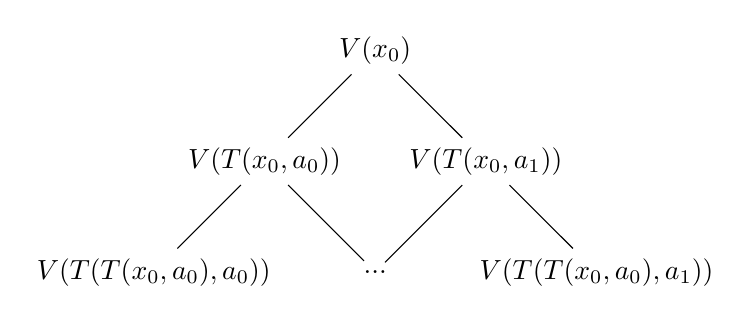
\begin{tikzpicture}
    [sibling distance=8em, level distance=4em]
    \node {$V(x_{0})$}
      child {node {$V(T(x_{0}, a_{0}))$}
        child {node {$V(T(T(x_{0}, a_{0}), a_{0}))$}}
        child {node {...}}
      }
      child {node {$V(T(x_{0}, a_{1}))$}
        child {node {}}
        child {node {$V(T(T(x_{0}, a_{0}), a_{1}))$}}
      };
  \end{tikzpicture}
\end{center}

Then, since you have the values of the base cases by definition, you can compute the values of the values that depend on the base cases, then the values that depend on those recursively until you reach your initial state again.

In this process, you find the value of $V(x)$ and $a(x)$ for every $x$ originating from the initial state.

To optimize this process, we would probably want to keep track of the values of $V(x)$ for every state $x$ in some sort of cache, recursion and memoization, sound familiar? This is exactly the idea behind the recursive method of doing DP.

\end{document}
